\documentclass[dvipsnames]{beamer}

\usepackage{xcolor}
\usepackage{lmodern}
\usepackage{minted}
\usepackage[utf8]{inputenc}
\usepackage{standalone}
\usepackage{tikz}
\usepackage{caption}
\usepackage{adjustbox}
\usepackage{upquote}
\usepackage{hyperref}
\usepackage{multirow}
\usepackage{booktabs}
\usepackage{array}
\usepackage{xspace}
\usetikzlibrary{mindmap,shadows,arrows,positioning,chains,fit,shapes}

\usetheme{metropolis}
\usemintedstyle{manni}

\definecolor{gmitblue}{RGB}{20,134,225}
\definecolor{gmitred}{RGB}{220,20,60}
\definecolor{gmitgrey}{RGB}{67,67,67}

\setbeamercolor{structure}{fg=gmitblue}
\setbeamercolor{frametitle}{fg=white, bg=gmitred}
\setbeamercolor{alerted text}{fg=gmitblue}

\newcommand{\hr}{\rule{\textwidth}{0.5pt}}

\renewcommand\footnoterule{}
\newcommand{\citeurl}[1]{\let\thefootnote\relax\footnotetext{\tiny \textcolor{gmitgrey}{\href{http://#1}{#1}}}}

\begin{document}
  \title{Emerging Technologies}
  \subtitle{}
  \author{ian.mcloughlin@gmit.ie}
  \date{}


  \begin{frame}
    \titlepage
  \end{frame}

  \begin{frame}
    \frametitle{Topics}
    \tableofcontents
  \end{frame}

  %!TEX root = slides.tex

\section{Languages}

\begin{frame}{Popular programming languages}
  \begin{description}
    \item[JavaScript] ``high-level, dynamic, untyped, and interpreted''
    \item[SQL] ``special-purpose programming language''
    \item[Java] ``general-purpose, concurrent, class-based, object-oriented''
    \item[C\#] ``multi-paradigm programming language''
    \item[PHP] `` server-side scripting''
    \item[Python] ``high-level, general-purpose, interpreted, dynamic''
    \item[C++] ``general-purpose, imperative, object-oriented and generic''
    \item[C] ``general-purpose, imperative''
    \item[Others] Node.js, AngularJS, Ruby, Objective-C (in order).
  \end{description}
  \citeurl{http://stackoverflow.com/research/developer-survey-2016}
\end{frame}


\begin{frame}{Kinds of programming languages}
  \begin{description}
    \item[Interpreted] Software interprets the language at runtime. 
    \item[Compiled] Software translates the language into machine code, which is then run.\\[1cm] 
    \item[Systems] Designed with operating system, device drivers development in mnid.
    \item[Applications] Designed with user applications development in mind.\\[1cm]
    \item[High-level] Abstration from the nitty-gritty computer details.
    \item[Imperative] Statements change the program state.
  \end{description}
\end{frame}

\begin{frame}{New languages}
  \begin{description}
    \item[Go] 2009 at Google. 
    \item[Rust] 2010 at Mozilla.
    \item[Swift] 2014 at Apple.
    \item[Hack] 2014 at Facebook, variant of PHP.
    \item[Scala] 2004 at EPFL (Martin Odersky).
    \item[Julia] 2012 at MIT.
    \item[Dart] 2011 at Google.
  \end{description}
\end{frame}


\begin{frame}{Styles in languages}
  \begin{figure}
    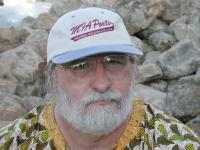
\includegraphics[height=3cm]{img/richard-gabriel.jpg}
  \end{figure}
  \begin{quote}
    I'm always delighted by the light touch and stillness of early programming languages.
    Not much text; a lot gets done.
    Old programs read like quiet conversations between a well-spoken research worker and a well studied mechanical colleague, not as a debate with a compiler.
    Who'd have guessed sophistication bought such noise? \\
    \hspace*\fill{\small--- Dick Gabriel}
  \end{quote}

  \citeurl{web.stanford.edu/class/ee380/Abstracts/100428-pike-stanford.pdf}
\end{frame}

\begin{frame}{People: Dennis Ritchie}
  \begin{figure}
    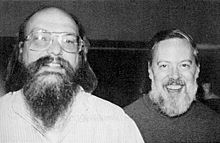
\includegraphics[height=3cm]{img/ritchie-thompson.jpg}
    \caption*{Dennis Ritchie 1941-2011 (right)}
  \end{figure}
  \begin{itemize}
    \item Helped Ken Thompson (left in above photo) to create UNIX.
    \item Created C, wrote book with Brian Kernighan.
  \end{itemize}
\end{frame}

\begin{frame}{People: Ken Thompson}
  \begin{figure}
    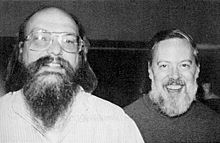
\includegraphics[height=3cm]{img/ritchie-thompson.jpg}
    \caption*{Ken Thompson (left)}
  \end{figure}
  \begin{itemize}
    \item Created UNIX.
    \item One of the creators of Go.
  \end{itemize}
\end{frame}


\begin{frame}{People: Brian Kernighan}
  \begin{figure}
    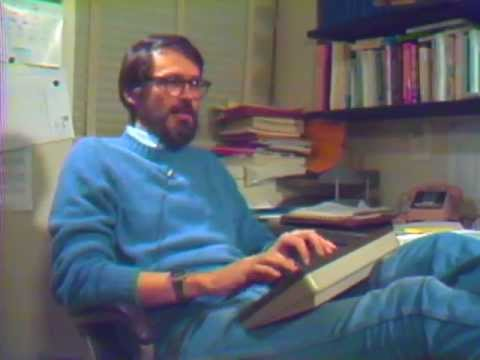
\includegraphics[height=3cm]{img/brian-kernighan.jpg}
  \end{figure}
  \begin{itemize}
    \item Wrote \emph{The C Programming Language} with Dennis Ritchie.
    \item Coined \mintinline{c}{Hello, world!}.
    \item Wrote \emph{The Go Programming Language} (with Alan Donovan).
  \end{itemize}
\end{frame}

\begin{frame}{People: Bjarne Stroustrup}
  \begin{figure}
    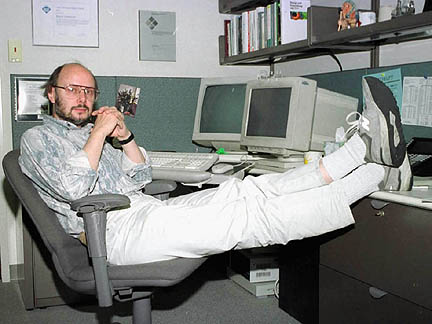
\includegraphics[height=3cm]{img/bjarne-stroustrup.jpg}
  \end{figure}
  \begin{itemize}
    \item Created C++.
    \item Coined \mintinline{c}{Hello, world!}.
    \item Wrote \emph{The Go Programming Language} (with Alan Donovan).
  \end{itemize}
\end{frame}

\begin{frame}{Places: Bell Labs}
  \begin{figure}
    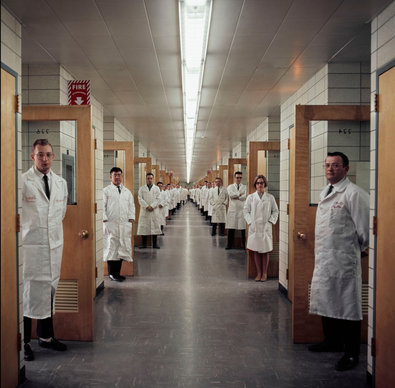
\includegraphics[height=3cm]{img/bell-labs.jpg}
  \end{figure}
  \begin{itemize}
    \item Pretty much set up by Alexander Graham Bell.
    \item Eight Nobel prizes, two Turing awards.
    \item Owned by Alcatel-Lucent, who were bought by Nokia.
  \end{itemize}
\end{frame}
  %!TEX root = slides.tex

\section{Go -- Getting Started}

\begin{frame}{Go features}
  \begin{description}
    \item[Concurrency] is builtin with light-weight goroutines, channels.  
    \item[Fast compiling] is a goal.
    \item[Packages] are easily managed and dependencies are quickly resolved.
    \item[Type inference] is available (sometimes).
    \item[C-like] in syntax. 
    \item[Tools] like go fmt and godoc are builtin. 
    \item[Garbage collection] is builtin.
  \end{description}
\end{frame}

\begin{frame}[fragile]{Hello, World!}
  \begin{minted}{go}
package main

import "fmt"

func main() {
  fmt.Println("Hello, world!")
}
  \end{minted}
  \citeurl{gobyexample.com/hello-world}
\end{frame}

\begin{frame}{go build}
  \begin{description}
    \item[go build] is the Go compiler.
    \item[go build hello.go] created an executable called hello (or hello.exe on windows).
    \item[Dependencies] are automatically built.
    \item[go run] is an alternative that also runs the program after.
    \item[Building] is fast in Go.
  \end{description}
  
  \citeurl{golang.org/cmd/go/}
\end{frame}


\begin{frame}[fragile]{Functions}
  \begin{minted}{go}
package main

import "fmt"

func add(x int, y int) int {
  return x + y
}

func main() {
  fmt.Println(add(42, 13))
}
  \end{minted}
  \citeurl{tour.golang.org/basics/4}
\end{frame}


\begin{frame}[fragile]{for loops}
  \begin{minted}{go}
package main

import "fmt"

func main() {
  sum := 0
  for i := 0; i < 10; i++ {
    sum += i
  }
  fmt.Println(sum)
}
  \end{minted}
  \citeurl{tour.golang.org/flowcontrol/1}
\end{frame}


\begin{frame}[fragile]{if and else}
  \begin{minted}{go}
func pow(x, n, lim float64) float64 {
  if v := math.Pow(x, n); v < lim {
    return v
  } else {
    fmt.Printf("%g >= %g\n", v, lim)
  }
  // can't use v here, though
  return lim
}
  \end{minted}
  \citeurl{tour.golang.org/flowcontrol/7}
\end{frame}

\begin{frame}[fragile]{Goroutines}
  \begin{minted}{go}
func say(s string) {
  for i := 0; i < 5; i++ {
    time.Sleep(100 * time.Millisecond)
    fmt.Println(s)
  }
}

func main() {
  go say("world")
  say("hello")
}
  \end{minted}
  \citeurl{tour.golang.org/concurrency/1}
\end{frame}
  %!TEX root = slides.tex

\section{Build tools}

\begin{frame}[fragile]{go help}
  \begin{minted}{bash}
> go help [command]
  \end{minted}
  \hr
\begin{description}
    \item[go help] prints out help for the go command
    \item[Optionally] you can provide another command line argument to to get help about a specific command.
  \end{description}
  
  \citeurl{golang.org/cmd/go}
\end{frame}


\begin{frame}[fragile]{GOPATH}
  \begin{minted}{bash}
> export GOPATH=/Users/john/go
  \end{minted}
  \hr
\begin{description}
    \item[GOPATH] is a variable that must be set properly to use go packages.
    \item[It's a list] of directories to look for packages in.
    \item[Directories] listed must have \mintinline{bash}{src}, \mintinline{bash}{pkg} and \mintinline{bash}{bin} subdirectories.
    \item[Colons] are used to separate the directories listed in GOPATH (but semicolons on Winodws). 
  \end{description}
  
  \citeurl{golang.org/cmd/go}
\end{frame}


\begin{frame}[fragile]{go fmt}
  \begin{minted}{bash}
> go fmt [-n] [-x] [packages]
  \end{minted}
  \hr
\begin{description}
    \item[go fmt] formats go code in a standard way.
    \item[gofmt] does the same, but reads and writes to and from stdin and stdout.
    \item[Tabs] are used to clean up the code, with one tab equal to 8 spaces.
    \item[Writing] code can be done in developers own style, then reformatted.
    \item[Reading] code is a bit easier, as there's a standard.
    \item[Diffs] are cleaner.
  \end{description}
  
  \citeurl{golang.org/cmd/go}
\end{frame}


\begin{frame}[fragile]{go get}
  \begin{minted}{bash}
> go get ... [-u] [build flags] [packages]
  \end{minted}
  \hr
\begin{description}
    \item[go get] downloads packages and installs them into the first entry in GOPATH.
    \item[Dependencies] are taken care of.
    \item[Source code] is put into the src subdirectory.
    \item[Object files] are put into the pkg directory.
    \item[Any exectuables] are put in bin.
  \end{description}
  
  \citeurl{golang.org/cmd/go}
\end{frame}

  %!TEX root = slides.tex

\section{Web Application Architectures}

\begin{frame}{What is a web application?}
  \begin{description}
    \item[Web applications] are web pages that are interactive, thanks to JavaScript.
    \item[JavaScript] is used to capture user events, and typically responds to them by firing off HTTP Requests in the background and changing the displayed resource based on the HTTP Response.
    \item[Resources] are typically generated on the fly by a web server, which usually interacts with a database.
    \item[LAMP] is an older architecture stack that follows this pattern.
    \item[MEAN] is a more modern stack.
  \end{description}
\end{frame}

\begin{frame}{Considerations}
  \begin{description}
    \item[Discoverable] Identifiable as applications, findable by search engines.
    \item[Linkable] Easily shareable via URLs, without requiring complex installation.
    \item[Progressive] Works for every user, regardless of browser choice.
    \item[Responsive] Fits any form factor: desktop, mobile, tablet, or whatever comes next.
    \item[Network] Works offline or on low quality networks.
  \end{description}
  \citeurl{developer.mozilla.org/en-US/Apps/Progressive}
\end{frame}

\begin{frame}{HTTP and CRUD}
  \tikzset{->-/.style={decoration={markings,mark=at position .5 with {\arrow{>}}},postaction={decorate}}}
  \tikzset{-<-/.style={decoration={markings,mark=at position .5 with {\arrow{<}}},postaction={decorate}}}
  \tikzstyle{rect} = [rectangle,fill=gmitblue,text width=5em,text centered,minimum height=16em,rounded corners,text=white]
  \begin{adjustbox}{max width={0.9\textwidth},center} 
    \begin{tikzpicture}[thick]

      \node [rect] (database) at (10,0) {Database};
      \node [rect] (webserver) at (5,0) {Web \\ Server};
      \node [rect] (client) at (0,0) {Client};

      \pgfmathsetmacro{\levela}{6em}
      \pgfmathsetmacro{\levelb}{2em}
      \pgfmathsetmacro{\levelc}{-2em}
      \pgfmathsetmacro{\leveld}{-6em}
      \pgfmathsetmacro{\diff}{0.3em}

      \path ([yshift={\levela+\diff}]webserver.west) edge[<-] node[anchor=south] {\footnotesize POST}     ([yshift={\levela+\diff}]client.east);
      \path ([yshift={\levela-\diff}]webserver.west) edge[->]                                             ([yshift={\levela-\diff}]client.east);
      
      \path ([yshift={\levela+\diff}]database.west) edge[<-] node[anchor=south] {\footnotesize CREATE}    ([yshift={\levela+\diff}]webserver.east);
      \path ([yshift={\levela-\diff}]database.west) edge[->]                                              ([yshift={\levela-\diff}]webserver.east);

      \path ([yshift={\levelb+\diff}]webserver.west) edge[<-] node[anchor=south] {\footnotesize GET}      ([yshift={\levelb+\diff}]client.east);
      \path ([yshift={\levelb-\diff}]webserver.west) edge[->]                                             ([yshift={\levelb-\diff}]client.east);
      
      \path ([yshift={\levelb+\diff}]database.west) edge[<-] node[anchor=south] {\footnotesize RETRIEVE}  ([yshift={\levelb+\diff}]webserver.east);
      \path ([yshift={\levelb-\diff}]database.west) edge[->]                                              ([yshift={\levelb-\diff}]webserver.east);

      \path ([yshift={\levelc+\diff}]webserver.west) edge[<-] node[anchor=south] {\footnotesize PUT}      ([yshift={\levelc+\diff}]client.east);
      \path ([yshift={\levelc-\diff}]webserver.west) edge[->]                                             ([yshift={\levelc-\diff}]client.east);
      
      \path ([yshift={\levelc+\diff}]database.west) edge[<-] node[anchor=south] {\footnotesize UPDATE}    ([yshift={\levelc+\diff}]webserver.east);
      \path ([yshift={\levelc-\diff}]database.west) edge[->]                                              ([yshift={\levelc-\diff}]webserver.east);

      \path ([yshift={\leveld+\diff}]webserver.west) edge[<-] node[anchor=south] {\footnotesize DELETE}   ([yshift={\leveld+\diff}]client.east);
      \path ([yshift={\leveld-\diff}]webserver.west) edge[->]                                             ([yshift={\leveld-\diff}]client.east);
      
      \path ([yshift={\leveld+\diff}]database.west) edge[<-] node[anchor=south] {\footnotesize DELETE}  ([yshift={\leveld+\diff}]webserver.east);
      \path ([yshift={\leveld-\diff}]database.west) edge[->]                                              ([yshift={\leveld-\diff}]webserver.east);

      \draw ([yshift={\levela+\diff}]webserver.west)  edge[dashed,draw=gray!60,->-] ([yshift={\levela+\diff}]webserver.east);
      \draw ([yshift={\levela-\diff}]webserver.west)  edge[dashed,draw=gray!60,-<-] ([yshift={\levela-\diff}]webserver.east);
      \draw ([yshift={\levelb+\diff}]webserver.west)  edge[dashed,draw=gray!60,->-] ([yshift={\levelb+\diff}]webserver.east);
      \draw ([yshift={\levelb-\diff}]webserver.west)  edge[dashed,draw=gray!60,-<-] ([yshift={\levelb-\diff}]webserver.east);
      \draw ([yshift={\levelc+\diff}]webserver.west)  edge[dashed,draw=gray!60,->-] ([yshift={\levelc+\diff}]webserver.east);
      \draw ([yshift={\levelc-\diff}]webserver.west)  edge[dashed,draw=gray!60,-<-] ([yshift={\levelc-\diff}]webserver.east);
      \draw ([yshift={\leveld+\diff}]webserver.west)  edge[dashed,draw=gray!60,->-] ([yshift={\leveld+\diff}]webserver.east);
      \draw ([yshift={\leveld-\diff}]webserver.west)  edge[dashed,draw=gray!60,-<-] ([yshift={\leveld-\diff}]webserver.east);

      \draw[dashed,draw=gray!60] ([yshift={\levela+\diff}]database.west)  -- ([yshift={\levela+\diff}]database.center) -- ([yshift={\levela-\diff}]database.center) -- ([yshift={\levela-\diff}]database.west);
      \draw[dashed,draw=gray!60] ([yshift={\levelb+\diff}]database.west)  -- ([yshift={\levelb+\diff}]database.center) -- ([yshift={\levelb-\diff}]database.center) -- ([yshift={\levelb-\diff}]database.west);
      \draw[dashed,draw=gray!60] ([yshift={\levelc+\diff}]database.west)  -- ([yshift={\levelc+\diff}]database.center) -- ([yshift={\levelc-\diff}]database.center) -- ([yshift={\levelc-\diff}]database.west);
      \draw[dashed,draw=gray!60] ([yshift={\leveld+\diff}]database.west)  -- ([yshift={\leveld+\diff}]database.center) -- ([yshift={\leveld-\diff}]database.center) -- ([yshift={\leveld-\diff}]database.west);


    \end{tikzpicture}
  \end{adjustbox}
\end{frame}

\begin{frame}{AMP}
  \tikzset{->-/.style={decoration={markings,mark=at position .5 with {\arrow{>}}},postaction={decorate}}}
  \tikzset{-<-/.style={decoration={markings,mark=at position .5 with {\arrow{<}}},postaction={decorate}}}
  \tikzstyle{rect} = [rectangle,fill=gmitblue,text width=5em,text centered,minimum height=16em,rounded corners,text=white]
  \begin{adjustbox}{max width={0.9\textwidth},center} 
    \begin{tikzpicture}[thick]

      \node [rect] (database) at (10,0) {MySQL};
      \node [rect] (webserver) at (5,0) {Apache \\ and PHP};
      \node [rect] (client) at (0,0) {Firefox};

      \pgfmathsetmacro{\levela}{6em}
      \pgfmathsetmacro{\levelb}{2em}
      \pgfmathsetmacro{\levelc}{-2em}
      \pgfmathsetmacro{\leveld}{-6em}
      \pgfmathsetmacro{\diff}{0.3em}

      \path ([yshift={\levela+\diff}]webserver.west) edge[<-] node[anchor=south] {\footnotesize POST}     ([yshift={\levela+\diff}]client.east);
      \path ([yshift={\levela-\diff}]webserver.west) edge[->]                                             ([yshift={\levela-\diff}]client.east);
      
      \path ([yshift={\levela+\diff}]database.west) edge[<-] node[anchor=south] {\footnotesize INSERT}    ([yshift={\levela+\diff}]webserver.east);
      \path ([yshift={\levela-\diff}]database.west) edge[->]                                              ([yshift={\levela-\diff}]webserver.east);

      \path ([yshift={\levelb+\diff}]webserver.west) edge[<-] node[anchor=south] {\footnotesize GET}      ([yshift={\levelb+\diff}]client.east);
      \path ([yshift={\levelb-\diff}]webserver.west) edge[->]                                             ([yshift={\levelb-\diff}]client.east);
      
      \path ([yshift={\levelb+\diff}]database.west) edge[<-] node[anchor=south] {\footnotesize SELECT}  ([yshift={\levelb+\diff}]webserver.east);
      \path ([yshift={\levelb-\diff}]database.west) edge[->]                                              ([yshift={\levelb-\diff}]webserver.east);

      \path ([yshift={\levelc+\diff}]webserver.west) edge[<-] node[anchor=south] {\footnotesize PUT}      ([yshift={\levelc+\diff}]client.east);
      \path ([yshift={\levelc-\diff}]webserver.west) edge[->]                                             ([yshift={\levelc-\diff}]client.east);
      
      \path ([yshift={\levelc+\diff}]database.west) edge[<-] node[anchor=south] {\footnotesize UPDATE}    ([yshift={\levelc+\diff}]webserver.east);
      \path ([yshift={\levelc-\diff}]database.west) edge[->]                                              ([yshift={\levelc-\diff}]webserver.east);

      \path ([yshift={\leveld+\diff}]webserver.west) edge[<-] node[anchor=south] {\footnotesize DELETE}   ([yshift={\leveld+\diff}]client.east);
      \path ([yshift={\leveld-\diff}]webserver.west) edge[->]                                             ([yshift={\leveld-\diff}]client.east);
      
      \path ([yshift={\leveld+\diff}]database.west) edge[<-] node[anchor=south] {\footnotesize DELETE}  ([yshift={\leveld+\diff}]webserver.east);
      \path ([yshift={\leveld-\diff}]database.west) edge[->]                                              ([yshift={\leveld-\diff}]webserver.east);

      \draw ([yshift={\levela+\diff}]webserver.west)  edge[dashed,draw=gray!60,->-] ([yshift={\levela+\diff}]webserver.east);
      \draw ([yshift={\levela-\diff}]webserver.west)  edge[dashed,draw=gray!60,-<-] ([yshift={\levela-\diff}]webserver.east);
      \draw ([yshift={\levelb+\diff}]webserver.west)  edge[dashed,draw=gray!60,->-] ([yshift={\levelb+\diff}]webserver.east);
      \draw ([yshift={\levelb-\diff}]webserver.west)  edge[dashed,draw=gray!60,-<-] ([yshift={\levelb-\diff}]webserver.east);
      \draw ([yshift={\levelc+\diff}]webserver.west)  edge[dashed,draw=gray!60,->-] ([yshift={\levelc+\diff}]webserver.east);
      \draw ([yshift={\levelc-\diff}]webserver.west)  edge[dashed,draw=gray!60,-<-] ([yshift={\levelc-\diff}]webserver.east);
      \draw ([yshift={\leveld+\diff}]webserver.west)  edge[dashed,draw=gray!60,->-] ([yshift={\leveld+\diff}]webserver.east);
      \draw ([yshift={\leveld-\diff}]webserver.west)  edge[dashed,draw=gray!60,-<-] ([yshift={\leveld-\diff}]webserver.east);

      \draw[dashed,draw=gray!60] ([yshift={\levela+\diff}]database.west)  -- ([yshift={\levela+\diff}]database.center) -- ([yshift={\levela-\diff}]database.center) -- ([yshift={\levela-\diff}]database.west);
      \draw[dashed,draw=gray!60] ([yshift={\levelb+\diff}]database.west)  -- ([yshift={\levelb+\diff}]database.center) -- ([yshift={\levelb-\diff}]database.center) -- ([yshift={\levelb-\diff}]database.west);
      \draw[dashed,draw=gray!60] ([yshift={\levelc+\diff}]database.west)  -- ([yshift={\levelc+\diff}]database.center) -- ([yshift={\levelc-\diff}]database.center) -- ([yshift={\levelc-\diff}]database.west);
      \draw[dashed,draw=gray!60] ([yshift={\leveld+\diff}]database.west)  -- ([yshift={\leveld+\diff}]database.center) -- ([yshift={\leveld-\diff}]database.center) -- ([yshift={\leveld-\diff}]database.west);


    \end{tikzpicture}
  \end{adjustbox}
\end{frame}
\end{document}